% !TeX spellcheck = it_IT

\section{Altri esempi}

\addcontentsline{toc}{subsection}{\protect\numberline{}Nascita della teoria dei grafi}
\subsection*{Nascita della teoria dei grafi}

La città di K\"onigsberg è attraversata dal fiume Pregel, nel quale sono presenti due isole collegate da 7 ponti in totale.\\

La domanda posta a Eulero fu: si può passare da tutti i ponti e tornare all'inizio? Ovvero, esiste un cammino che passa per tutti gli archi (ponti) del grafo per poi tornare al nodo iniziale?\\

Le due isole diventano 2 vertici e le sponde altri 2. Al giorno d'oggi sarebbe chiamato "multigrafo", avendo più lati incidenti sugli stessi due vertici, ma il problema rimane lo stesso.\\

Se volessimo formalizzare il problema nella terminologia moderna: dato un multigrafo, esiste un circuito che passa per tutti i lati? Si chiama "circuito Euleriano" (indovina perché).\\

\addcontentsline{toc}{subsubsection}{\protect\numberline{}Teorema di Eulero}
\paragraph{Teorema di Eulero:} \textbf{Esiste} un \textbf{circuito Euleriano iff} il grafo è connesso (ovviamente) e \textbf{tutti i vertici hanno grado pari}.\\

Come si \textbf{costruisce un circuito}, a partire \textbf{da un grafo con vertici di grado pari}? \\
Partendo da un qualsiasi vertice $x_0$ e si percorre un qualunque lato, arrivando ad $x_1$, il quale avrà almeno un altro lato uscente (avendo esso grado pari), che arriva ad $x_2$, e la cosa si ripete.\\
Nel caso si crei un ciclo prima di toccare tutti i lati vuol dire che questo ha almeno 4 lati incidenti e quindi si può continuare.\\
Se si torna ad $x_0$ prima di toccare tutti i lati, si ricomincia senza considerare i lati già visti.\\

\newpage

\addcontentsline{toc}{subsection}{\protect\numberline{}Handshaking Lemma}
\subsection*{Handshaking Lemma}
"Lemma delle strette di mano", se un gruppo di persone si stringono la mano, il numero di persone che stringono la mano a un numero dispari di persone sono in quantità pari.\\

\addcontentsline{toc}{subsubsection}{\protect\numberline{}Teorema}
\paragraph{Teorema:} In un grafo $G=(V,E)$, il numero di vertici di grado ($d()$) dispari è pari.\\

\begin{proof}
	Sommando i gradi di tutti i vertici
	$$ \sum_{x \in V} d(x) = 2m $$
	In questo modo ogni lato viene contato 2 volte, quindi è pari 2 volte il numero di lati $m$. $2m$ è ovviamente pari, e i nodi con grado pari possono non essere considerati ai fini della parità (se tolgo o aggiungo un numero pari la parità non cambia), quindi i nodi con grado dispari devono essere pari, altrimenti la somma potrebbe non essere pari.\\
\end{proof}

% End L9

\newpage

\subsection{Problema del Traveling Salesman (TSP)}
Avendo un insieme di città collegate da strade bidirezionali (grafo pesato) un commesso vuole passare per tutte le città una e una sola volta, facendo un percorso di lunghezza minima per poi tornare a casa (vuole fare il giro).\\

Definizione: 
\begin{itemize}
	\item \textbf{Input}: un \textbf{grafo non orientato} $G = (V,E)$ con delle \textbf{lunghezze} $[\delta_e]_{e \in E}$ per ogni \textbf{lato}
	
	\item \textbf{Soluzioni ammissibili}: circuiti che passano per ogni vertice esattamente una volta (\textbf{circuito hamiltoniano})
	
	\item \textbf{Funzione obiettivo}: la \textbf{lunghezza} del circuito
	
	\item \textbf{Tipo}: minimizzazione, $\min$
\end{itemize}


Non è detto che il circuito hamiltoniano esista.\\

Questo problema è \textbf{equivalente al TSP su clique} (quindi su un grafo fully connected). Per usare un algoritmo che funziona solo su clique per grafi generici basta aggiungere i lati mancanti con un peso molto alto (più di ogni possibile cammino tra lati tendenzialmente), in modo che non vengano mai scelti, se la soluzione passa per uno dei lati "finti" nel grafo originale non c'è un circuito hamiltoniano.\\

Per questo da qui in poi verrà \textbf{presupposto che i grafi siano clique} $G = K_n$ (notazione per una clique di $n$ nodi).\\

\newpage

\paragraph{TSP Metrico:} Un TSP Metrico ha come proprietà:
\begin{itemize}
	\item $G$ è una clique 
	\item $\forall x,y,z$, $\delta_{xy} \leq \delta_{xz} + \delta_{zy}$ (disuguaglianza triangolare)
\end{itemize}

\nn

\paragraph{Ingredienti mancanti: } Due concetti che serviranno per l'algoritmo vero e proprio:
\begin{itemize}
	\item \textbf{Minimum spanning tree}: dato un grafo pesato connesso $G = (V,E)$ trovare un albero di copertura (che tocca tutti i vertici) di peso totale minimo. Risolvibile in tempo polinomiale (es. Algoritmo di Kruskal).\\
	
	\item \textbf{Minimum weight perfect matching}: Data una clique pesata un numero pari di vertici trovare un matching perfetto (completo) di peso minimo. Risolvibile esattamente in tempo polinomiale (Blossom algorithm)
\end{itemize}

Ora possiamo cucinare.\\

\newpage

\subsubsection{Algoritmo di Cristophides}

Algoritmo \textbf{per il TSP metrico}:
\begin{itemize}
	\item Input: $G = (V,E)$ clique, con pesi $[\delta_e]_{e \in E}$ che sono una metrica
\end{itemize}

\textbf{Passaggi} dell'algoritmo:
\begin{enumerate}
	\item \textbf{Troviamo} un \textbf{minimum spanning tree} $T$.\\
	
	\item Sia $D$ l'insieme dei \textbf{vertici di grado dispari in} $T$. Per Handshaking Lemma sappiamo che $D$ ha \textbf{cardinalità pari}.\\
	
	\item Scegliamo un \textbf{minimum weight perfect matching} $M$ \textbf{sui nodi presenti in} $D$ (sicuramente presente, dato che quei nodi fanno parte di una clique e sono pari).\\ 
	
	\item Il perfect matching potrebbe riusare lati dell'albero, se il lato compare sia nel MST che nel matching bisognerà andare a considerare un multigrafo. \\
	Sia $H = T \dot{\cup} M$ (unione tenendo le ripetizioni). Tutti i vertici di $H$ avranno grado pari, in quanto tutti quelli che avevano grado dispari hanno ricevuto un lato bonus dal matching.\\
	
	\item Avendo tutti grado pari si può usare il teorema di Eulero, quindi \textbf{troviamo un circuito euleriano} $\pi$.\\
	
	\item Ma questo può passare per lo stesso vertice più di una volta, si tratta di un circuito euleriano, noi lo vogliamo hamiltoniano. Quindi \textbf{trasformo $\pi$ in un circuito hamiltoniano} $\tilde \pi$. Per farlo bisogna "strozzare i cappi", quando $\pi$ passa per un nodo già preso, lo salto, tanto siamo in una clique, quindi al posto di fare il giro $x, y, z$, se ho già preso prima $y$, posso fare direttamente $x,z$.\\
\end{enumerate}

Insomma, seguo il circuito euleriano ma salto i nodi visitati più volte, rendendolo un circuito hamiltoniano. Questo è l'output.\\

\newpage

%\addcontentsline{toc}{subsubsection}{\protect\numberline{}Lemma 1}
\paragraph{Lemma 1:} $\delta (T) \leq \delta^\ast$, la somma dei pesi presenti nel MST è minore il peso del circuito hamiltoniano ottimo.\\

\begin{proof}
	Sia $\pi^\ast$ un TSP ottimo. Se da $\pi^\ast$ togliamo un lato otteniamo un albero di copertura minimo (da un circuito, se tolgo un lato non ho più cicli, quindi ho un albero), quindi 
	$$ \delta (T) \leq \delta^\ast - \delta_e \leq \delta^\ast $$
\end{proof}

%\addcontentsline{toc}{subsubsection}{\protect\numberline{}Lemma 2}
\paragraph{Lemma 2:} $\delta(M) \leq \frac{1}{2} \delta^\ast$.\\

\begin{proof}
	Sia $\pi^\ast$ is TSP ottimo. Dentro questo ci saranno anche i vertici di grado dispari presenti in $D$ che deve coprire il matching $M$.\\
	
	Prendendo un circuito tra elementi di $D$ (vertici di grado dispari) e chiamandolo $\overline{\pi}^\ast$, ma questo ovviamente 
	$$\overline{\pi}^\ast \leq \delta (\pi^\ast) $$
	Sto saltando dei pezzi dal circuito originale, sicuramente è meno.\\
	
	Dividiamo i lati di $\overline{\pi}^\ast$ in due insiemi $M_1$ e $M_2$ alternati. Ognuno di questi due gruppi di lati è un perfect matching su $D$, ma sappiamo che $M$  è il minimum perfect matching, quindi:
	$$ \delta (M) \leq \delta (M_1) $$
	$$ \delta (M) \leq \delta (M_2) $$
	
	Di conseguenza
	$$ 2 \delta (M) \leq \delta (M_1) + \delta (M_2)  = \delta (\overline{\pi}^\ast) \leq \delta (\pi^\ast)$$
	$$ \implies \delta (M) \leq \frac{1}{2} \delta^\ast$$
\end{proof}

\addcontentsline{toc}{subsubsection}{\protect\numberline{}Teorema}
\paragraph{Teorema:} L'algoritmo di Cristophides fornisce una \textbf{$3/2$-approssimazione per il TSP metrico}.\\

\begin{proof}
	$$\delta(\pi) = \delta (T) + \delta(M)$$
	Usando i due lemmi:
	$$ \delta (T) + \delta (M) \leq \delta^\ast + \frac{1}{2} \delta^\ast $$
	$$ \implies \delta (\pi) \leq \frac{3}{2} \delta ^\ast $$
	
	Per la triangolare (durante la trasformazione prendo solo lati in meno, mai in più):
	$$ \delta (\tilde \pi) \leq \delta (\pi) \leq \frac{3}{2} \delta^\ast $$
\end{proof}

\addcontentsline{toc}{subsubsection}{\protect\numberline{}Tightness}
\paragraph{Tightness:} l'analisi è stretta, esistono input per cui l'algoritmo restituisce $\sfrac{3}{2} \delta^\ast$.\\

\begin{proof}
	$n \in \mathbb{N}$ pari e $\epsilon \in (0,1)$. Prendiamo $n$ nodi, li colleghiamo in un cammino in fila e tutti questi lati hanno lunghezza $1$. \\
	Aggiungo lati da 1 a 3, da 2 a 4, da 3 a 5, da 5 a 7, tra tutti i pari e tra tutti i dispari, ognuno di lunghezza $1 + \epsilon$.\\
	
	Sia $K_{n,\epsilon}$ la clique ottenuta aggiungendo tutti i lati mancanti, ognuno dei quali con lunghezza pari al cammino minimo tra i due vertici collegati. Ovviamente è metrica in quanto per costruzione rispetta la triangolare.\\
	
	\begin{center}
		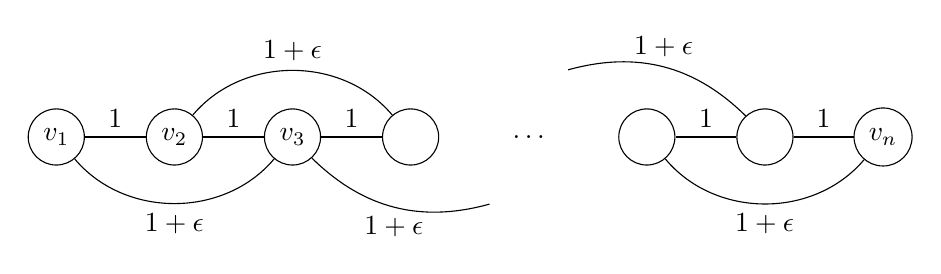
\begin{tikzpicture}[scale=1.5]
			\node[draw, circle] (1) at (0,0) {$v_1$};
			\node[draw, circle] (2) at (1,0) {$v_2$};
			\node[draw, circle] (3) at (2,0) {$v_3$};
			\node[draw, circle] (4) at (3,0) {\phantom{$v_1$}};
			\node (4.5) at (4,0) {$\dots$};
			\node (up) at (4.25, 0.55) {};
			\node (down) at (3.75, -0.55) {};
			\node[draw, circle] (5) at (5,0) {\phantom{$v_1$}};
			\node[draw, circle] (6) at (6,0) {\phantom{$v_1$}};
			\node[draw, circle] (7) at (7,0) {$v_n$};
			
			\draw[-] (1) to node[midway, above] {$1$} (2);
			\draw[-] (2) to node[midway, above] {$1$} (3);
			\draw[-] (3) to node[midway, above] {$1$} (4);
			\draw[-] (5) to node[midway, above] {$1$} (6);
			\draw[-] (6) to node[midway, above] {$1$} (7);
			
			\draw[-, bend right=50] (1) to node[midway, below] {$1 + \epsilon$} (3);
			\draw[-, bend right=50] (5) to node[midway, below] {$1 + \epsilon$} (7);
			
			\draw[-, bend right=30] (3) to node[below] {$1 + \epsilon$} (down);
			\draw[-, bend left=30] (up) to node[above] {$1 + \epsilon$} (6);
			
			\draw[-, bend left=50] (2) to node[midway, above] {$1 + \epsilon$} (4);
			
		\end{tikzpicture}
	\end{center}
	
	
	\newpage
	
	Cristophides sceglie il MST, che in questo caso saranno tutti i lati di lunghezza $1$. $T$ prende tutti gli $n-1$ lati di lunghezza $1$, quindi 
	$$\delta (T) = n-1$$
	
	Gli unici vertici di grado dispari sono il primo e l'ultimo, quindi il minimum perfect matching sarà il lato tra $v_1$ e $v_n$, il quale sarà pari al cammino minimo tra i due ovvero tutti gli $1 + \epsilon$ possibili, più l'ultimo lato:
	$$ \delta(M) = (1 + \epsilon) \frac{n}{2} + 1$$
	
	Il cammino hamiltoniano coinciderà con quello euleriano quindi:
	$$ \delta = \delta (T) + \delta (M) = n-1 + (1 + \epsilon) \frac{n}{2} + 1 = \frac{3}{2} n + \epsilon \frac{n}{2} $$
	
	Ma il circuito ottimo è prendere due lati da 1 affianco a primo e ultimo nodo, poi tutti i lati da $1 + \epsilon$, quindi il totale: 
	$$ \delta^\ast = (1+ \epsilon)n + 2 $$
	
	Quindi il rapporto di approssimazione diventa: 
	$$ \frac{\delta}{\delta^\ast} = \frac{\frac{3}{2}n + \epsilon \frac{n}{2}}{ (1 + \epsilon) n + 2} \rightarrow \frac{3}{2}$$
	Tende a $3/2$ per $n \rightarrow +\infty$ e $\epsilon \rightarrow 0$.\\
\end{proof}

\newpage

% End L10

\subsubsection{Inapprossimabilità del TSP}

TSP Metrico è approssimabile, \textbf{quello generale no}.\\

\addcontentsline{toc}{subsubsection}{\protect\numberline{}Teorema}
\paragraph{Teorema:} Non esiste $\alpha>1$ tale che TSP sia $\alpha$-approssimabile (se $\mathcal{P} \neq \mathcal{NP}$). Il problema sta fuori da APX.\\

\begin{proof}
	Fact: Il problema di \textbf{decidere se un grafo ammetta un circuito hamiltoniano} è $\mathcal{NP}$-Completo (problema di decisione).\\
	
	Supponiamo per assurdo di \textbf{avere un algoritmo $\alpha$-approssimante per TSP}. \\
	
	Supponendo di avere un grafo $G=(V,E)$ e voler sapere se questo grafo ha un circuito hamiltoniano. Per \textbf{trasformarlo in un'istanza di TSP}, dobbiamo \textbf{aggiungere pesi} e \textbf{trasformarlo in una clique}
	$$ G' = \left(V, \left(
	\begin{array}{c}
		V\\
		2
	\end{array}
	\right), d \right)$$
	
	Bisogna aggiungere le \textbf{distanze}, dove
	$$ 
	d(x,y) = \begin{cases}
		1 & \text{ se } \; \{x,y\} \in E \\
		\lceil \alpha n \rceil + 1 & \text{ altrimenti}
	\end{cases}
	$$
	
	Si tratta di una clique, quindi per forza ci deve essere un circuito hamiltoniano su $G'$, ma se $G$ \textbf{ammetteva} un circuito hamiltoniano a sua volta, allora $G'$ ne ha uno con lunghezza $\leq n$.\\
	Se $G$ \textbf{non ha un circuito hamiltoniano}, qualunque circuito hamiltoniano viene trovato \textbf{su} $G'$ ha \textbf{lunghezza} $\geq \lceil \alpha n\rceil + 1$.\\
	
	\newpage
	
	Diamo $G'$ come \textbf{input dell'algoritmo} $\alpha$-approssimante per TSP, questo \textbf{emetterà} nei casi:
	\begin{itemize}
		\item $G$ ha un c.H.: l'algoritmo emette un output $\leq \alpha n$ (dato che si tratta di una $\alpha$-approssimazione)
		\item $G$ non ha un c.H.: l'algoritmo emette un output $\geq \lceil \alpha n \rceil + 1$
	\end{itemize}
	
	Quindi possiamo avere output $\leq \alpha n$ e  $\geq \lceil \alpha n \rceil + 1$, ma \textit{è possibile che questi due intervalli si sovrappongano}?
	$$ \alpha n \geq \lceil \alpha n \rceil + 1 $$
	$$ \implies \alpha \geq \frac{\lceil \alpha n \rceil + 1}{n} \geq \frac{\alpha n + 1}{n} = \alpha + \frac{1}{n}$$
	$$ \alpha \geq \alpha + \frac{1}{n}$$
	
	Quindi sono \textbf{intervalli sempre disgiunti} e di conseguenza le soluzioni sono ben distinte.\\
	
	Questo vorrebbe dire risolvere il problema di decidere se un grafo ammetta un circuito hamiltoniano efficientemente, che sappiano non essere possibile essendo in $\NP$.\\
\end{proof}

\newpage